\section{Usage Scenarios}
\label{sec:3}

This section introduces in detail how to use the framework for common usage scenarios.

\subsection{Bitcoin Trading}

In this example, we demonstrate how to use the framework to experiment Bitcoin trading with the \emph{MovingAverageTrader} on live market data. The component graph of this application is as follows:

\noindent
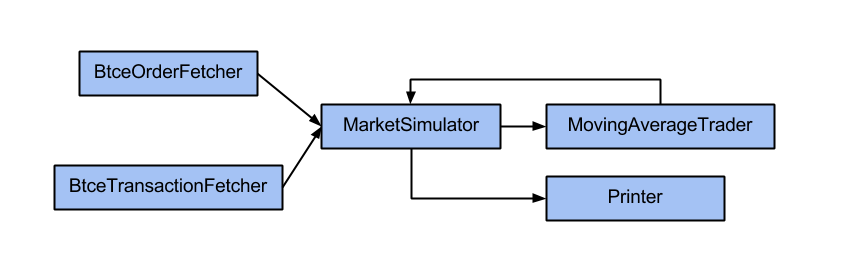
\includegraphics[width=\textwidth]{img/examples/btce}

The BTC-E fetchers get orders and transactions from \url{btc-e.com}, feed them to the market simulator. The market simulator generates transactions based on the bid and ask orders from the trader. The trader sends bid or ask orders to the market simulator based on the transactions received from the market simulator. The printer prints information about the market in the console.

\subsection{Forex Trading}

In this example, we demonstrate how to use the framework to experiment Forex trading with the \emph{MovingAverageTrader} on live Forex data. The component graph of this application is as follows:

\noindent
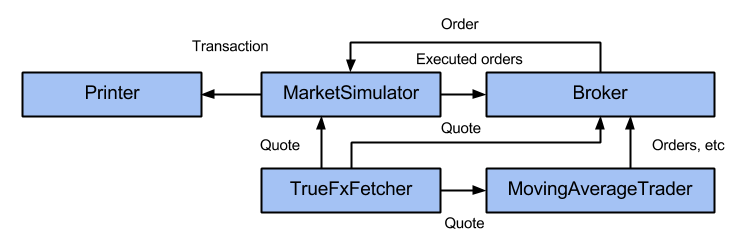
\includegraphics[width=\textwidth]{img/examples/forex-live}

In the component graph above, the fetcher gets live quotes data from \url{webrates.truefx.com}, and feeds them into the market simulator, trader and broker.

The trader makes sell and buy decisions based on the quotes received from the fetcher, and send them to the broker.

The broker receives orders from the trader, and forward them into the market simulator on behalf of the trader. Note that the usage of broker is optional, it's used here only for illustrating purpose.

The market simulator generates transactions based on the orders from traders.

\subsection{Replay}

Forex or Bitcoin trading with a single trader from history data

\subsection{Simulation with Multiple Traders}

Multiple trader simulation in a virtual market.
